% \documentclass{article}
\documentclass[fleqn]{article}
\usepackage{amsmath}
\usepackage{enumitem}
\usepackage{import}
\subimport*{../assignment-2/}{macro}

\setlength\parindent{20px}
\setlength{\mathindent}{20pt}

\begin{document}
\title{Homework \#3}
\author{Aaron Chen / aaronyc}
\date{}
\maketitle

% ------ setting ------

\subsection*{A1. Conceptual Questions}

\begin{enumerate}[label=(\alph*)]
\item
False. Neural networks are non-convex (e.g. multilayer cross-entropy loss). Gradient descent can still be run, but it only has stronger optimization guarantees for convex objectives, so it is not guaranteed to find the global optimum.

\item
False. Initializing all weights to zero fails to break symmetry: neurons in the same layer get the same gradients and remain identical during training. Random initialization is preferred because it lets different neurons learn different features.

\item
True. Examples of non-linear activation functions: Sigmoid, ReLU, tanh.

\item
False. Backpropagation reuses intermediate values from the forward pass and computes all gradients efficiently with the chain rule. The backward pass is usually only a constant-factor more expensive than the forward pass, not prohibitively larger.

\item
False. Neural networks are flexible, but they are not always the best choice. For example, in settings where interpretability is important, simpler models such as linear or logistic regression may be preferable.
\end{enumerate}

% ---------------------

\subsection*{A2. Kernels: RBF Feature Map}

\begin{align*}
\phi(x) \cdot \phi(x')
&= \sum_{i=0}^{\infty}
\left(\frac{1}{\sqrt{i!}}e^{-x^2/2}x^i\right)
\left(\frac{1}{\sqrt{i!}}e^{-{x'}^2/2}{x'}^i\right) \\
&= e^{-x^2/2}e^{-{x'}^2/2}
\sum_{i=0}^{\infty}\frac{(xx')^i}{i!} \\
&= e^{-x^2/2}e^{-{x'}^2/2}e^{xx'} \\
&= e^{-\frac{x^2}{2}-\frac{{x'}^2}{2}+xx'} \\
&= e^{-\frac{x^2-2xx'+{x'}^2}{2}} \\
&= e^{-\frac{(x-x')^2}{2}} \\
&= K(x,x')
\end{align*}

\[
K(x,x') = e^{-\frac{(x-x')^2}{2}}
\]

% ---------------------

\subsection*{A3. Kernel Ridge Regression}

\begin{enumerate}[label=(\alph*)]
\item
The selected hyperparameters are:

\begin{center}
\begin{tabular}{c|c|c|c}
Kernel & $d$ & $\gamma$ & $\lambda$ \\
\hline
Polynomial & $16$ & -- & $4.281332398719396 \times 10^{-5}$ \\
RBF & -- & $10.541635373659384$ & $0.00206913808111479$
\end{tabular}
\end{center}

\item
Polynomial kernel:
\begin{center}
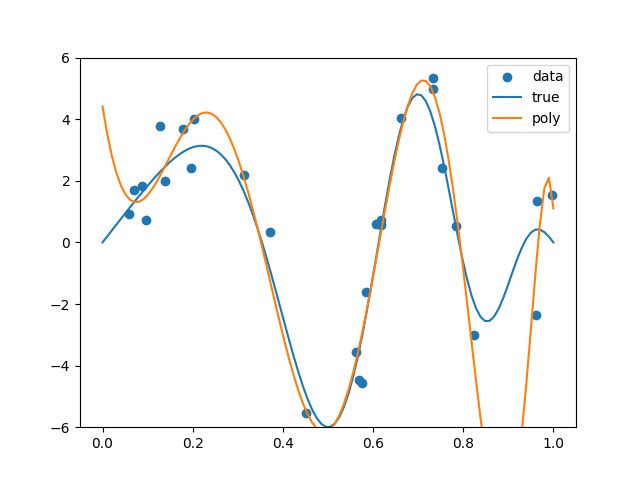
\includegraphics[width=0.8\textwidth]{hw3-A/kernel_poly.png}
\end{center}

RBF kernel:
\begin{center}
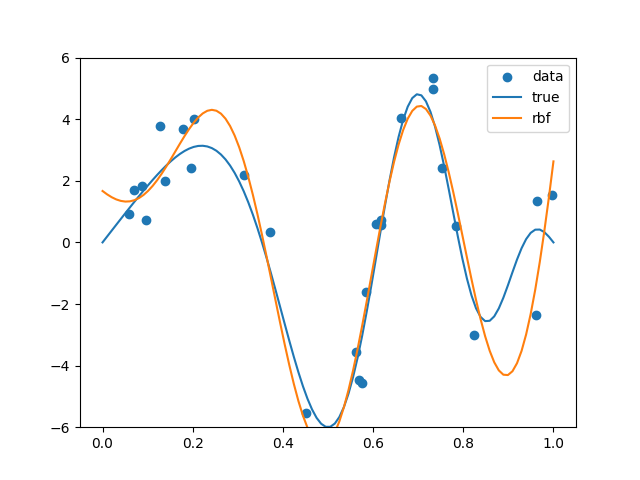
\includegraphics[width=0.8\textwidth]{hw3-A/kernel_rbf.png}
\end{center}
\end{enumerate}

% ---------------------

\subsection*{A4. Introduction to PyTorch}

\begin{enumerate}[label=(\alph*)]
\setcounter{enumi}{1}
\item
Cross-entropy loss:
\begin{center}
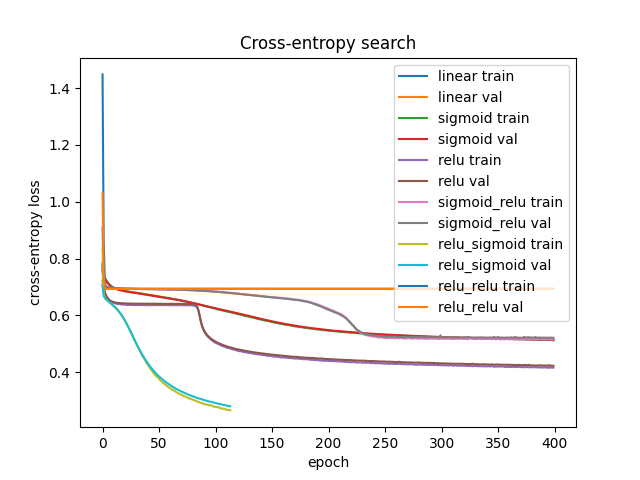
\includegraphics[width=0.8\textwidth]{hw3-A/crossentropy_loss.png}
\end{center}

Mean squared error loss:
\begin{center}
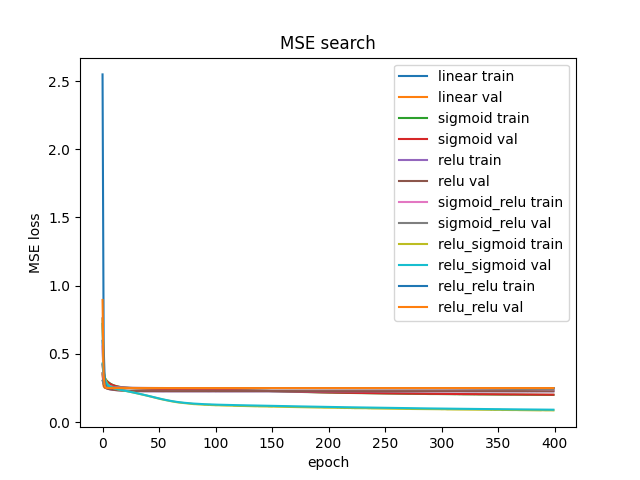
\includegraphics[width=0.8\textwidth]{hw3-A/mse_loss.png}
\end{center}

\item
For cross-entropy loss, the best-performing architecture is ReLU then Sigmoid.

\[
\text{Test accuracy} = 0.9184
\]

\begin{center}
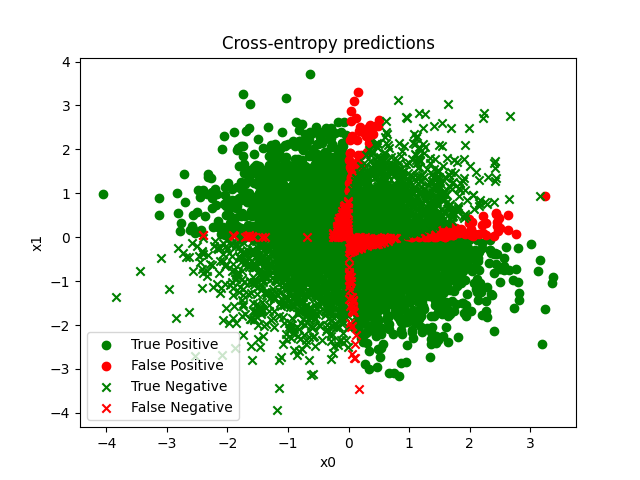
\includegraphics[width=0.8\textwidth]{hw3-A/crossentropy_predictions.png}
\end{center}

For mean squared error loss, the best-performing architecture is ReLU then Sigmoid.

\[
\text{Test accuracy} = 0.9092
\]

\begin{center}
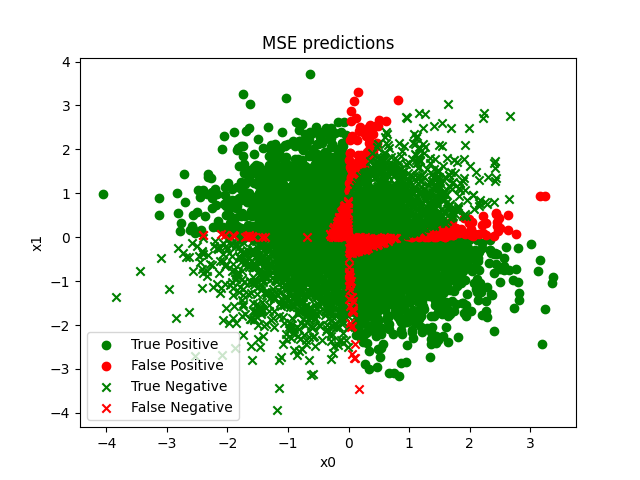
\includegraphics[width=0.8\textwidth]{hw3-A/mse_predictions.png}
\end{center}
\end{enumerate}

% ---------------------

\subsection*{A5. Neural Networks for MNIST}

\begin{enumerate}[label=(\alph*)]
\item
Wide shallow network:

\begin{center}
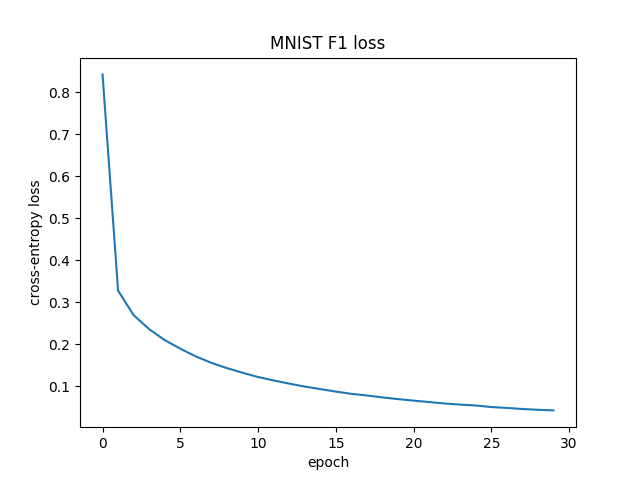
\includegraphics[width=0.8\textwidth]{hw3-A/mnist_f1_loss.png}
\end{center}

\[
\begin{array}{l}
\text{Test accuracy} = 0.9736 \\
\text{Test loss} = 0.0871247056722641
\end{array}
\]

\item
Narrow deeper network:

\begin{center}
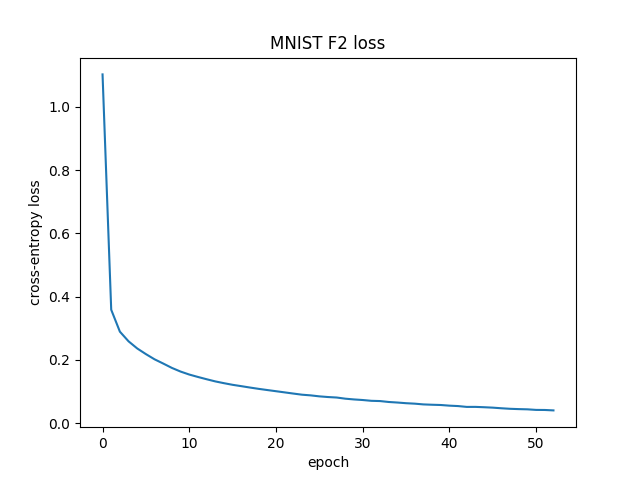
\includegraphics[width=0.8\textwidth]{hw3-A/mnist_f2_loss.png}
\end{center}

\[
\begin{array}{l}
\text{Test accuracy} = 0.965 \\
\text{Test loss} = 0.13156537783145905
\end{array}
\]

\item
\[
\begin{array}{l}
\#\text{parameters for wide shallow network} = 50890 \\
\#\text{parameters for narrow deeper network} = 26506
\end{array}
\]

The wide shallow network has more parameters and slightly better test accuracy.
The narrow deeper network uses about half as many parameters, but its accuracy is only slightly lower.
\end{enumerate}

% ---------------------

\subsection*{A6. Multinomial Logistic Regression}

\begin{enumerate}[label=(\alph*)]
\item
For one example $(x_i,y_i)$,
\[
L_i(W) = -\log p(y_i \mid x_i; W)
\]

\begin{align*}
L_i(W)
&= -\log\round{
\frac{\exp(W_{y_i}^\top x_i)}
{\sum_{\ell=1}^{k}\exp(W_\ell^\top x_i)}
} \\
&= -W_{y_i}^\top x_i
+ \log\round{\sum_{\ell=1}^{k}\exp(W_\ell^\top x_i)}
\end{align*}

\begin{align*}
\nabla_{W_j} L_i(W)
&= -\mathbf{1}\curly{j=y_i}x_i
+ \frac{\exp(W_j^\top x_i)}
{\sum_{\ell=1}^{k}\exp(W_\ell^\top x_i)}x_i \\
&= \round{p(y=j\mid x_i;W)-\mathbf{1}\curly{j=y_i}}x_i
\end{align*}

\item
The results are:

\begin{center}
\begin{tabular}{c|c|c}
Loss & Training accuracy & Test accuracy \\
\hline
\texttt{J\_loss} & $0.9290$ & $0.9245$ \\
\texttt{L\_loss} & $0.9280$ & $0.9233$
\end{tabular}
\end{center}

\texttt{J\_loss} plots:
\begin{center}
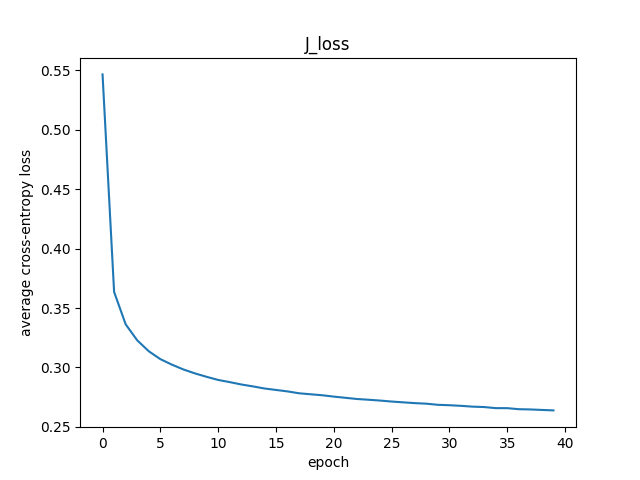
\includegraphics[width=0.8\textwidth]{hw3-A/multinomial_J_loss.png}
\end{center}

\texttt{L\_loss} plots:
\begin{center}
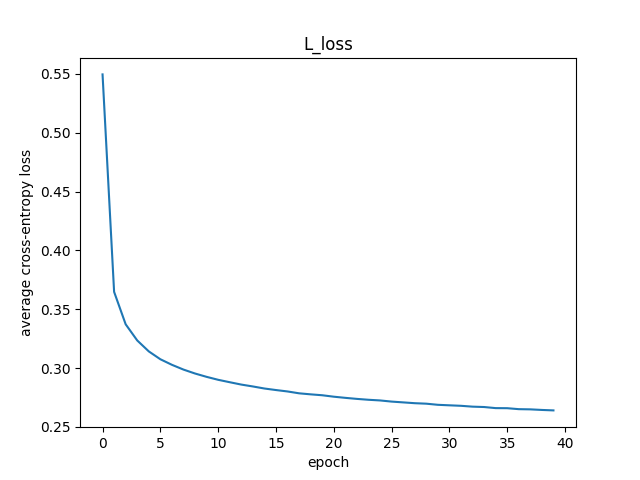
\includegraphics[width=0.8\textwidth]{hw3-A/multinomial_L_loss.png}
\end{center}
\end{enumerate}

% ---------------------

\end{document}
